\twocolumn[
\title{\bf Fancy Jabde LaTeX Template for Academic Tom Foolery}
\author{
Author A. One$^{1,2}$,
Author B. Two$^{1}$,
}
\date{April 1st 2022}
% List of institutions
\maketitle
$^{1}$Waste of Money Department, University of Somewhere, Place, City, Country \\
$^{2}$Department Academic Overreach, Cranberry Lemon University, Pittsburgh, PA USA
\begin{psummary}
Write a thrilling and catching abstract here.
\end{psummary}
\vspace{2mm}
]
\fancypagestyle{firstpage}{%
  \lhead{Cranberry-Lemon}
  \rhead{Journal of Astrological Big Data Ecology}
}
\thispagestyle{firstpage}

% The introduction
\section{Introduction}

Wooh, time to write a made up paper

\subsection{Background}

In order to understand this study you should understand.

\begin{enumerate}
    \item Thing one.
    \item Thing two\footnote{With a footnote}.
    \item Thing Three.
\end{enumerate}


\section{Methodology} 

In order to invent this thing or analyze this data, we're going to need to use the equation below.

\begin{equation}
Heuristic_\alpha(x) = \sqrt{\sum{All of the things}},
\end{equation}

Of course we trust that equation because of the work done in \cite{OnlineRef1} which may or may not agree with the dude that wrote \cite{ArticleRef}.

\section{Another Section}

I don't know, you could have a boring data collection bit here, or an architecture, or something. I'm sure it'll be mostly filler.

\section{Filler Section 2}

As shown in figure \ref{fig:Freud}, Freud is not displaying Penis envy by holding a cigar.

\begin{figure}[h]
    \centering
    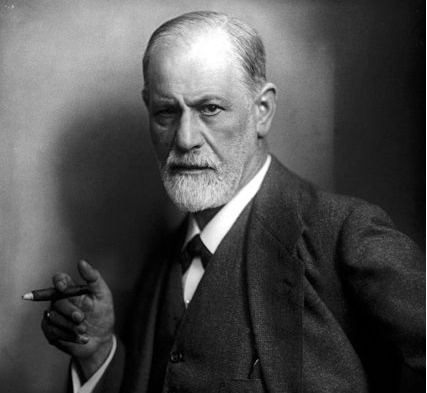
\includegraphics[width=\columnwidth]{\projectpath figs/Freud.PNG}
    \vspace{0.1in}
    \caption{Freud Holding just a cigar.}
    \label{fig:Freud}
    \vspace{0.1in}
\end{figure}

I swear it's just a cigar.

\section{Discussion and Results}

According to all of this data and our unbiased analysis, all of our beliefs have been validated. Just check out Table \ref{table:1}.

\begin{table}[h!]
\vspace{0.1in}
\begin{center}
\begin{tabular}{||c c c c||} 
 \hline
 Col1 & Col2 & Col2 & Col3 \\ [0.5ex] 
 \hline\hline
 1 & 6 & 87837 & 787 \\ 
 \hline
 2 & 7 & 78 & 5415 \\
 \hline
 3 & 545 & 778 & 7507 \\
 \hline
 4 & 545 & 18744 & 7560 \\
 \hline
 5 & 88 & 788 & 6344 \\ [1ex] 
 \hline
\end{tabular}
\vspace{0.1in}
\caption{Table to prove how right you are.}
\label{table:1}
\end{center}
\end{table}


Wow, what astounding results!

\section{Conclusion}

In conclusion, I am very smart

\section{Acknowledgements}

I did this all by myself, so I'm kinda awesome. But I guess I hocked and edited this template from the cowshed article so thanks for that William Roper

\begingroup
\setlength\bibitemsep{0pt}
\setlength\bibnamesep{0pt}
\printbibliography[heading=subbibliography]
\endgroup

%when translating non-inline equations into Wordpress, use the code below
%<p align="center"> $latex \displaystyle \mathop{\mathbb E}_{x\sim X} f(x):= 1 \ \ \ \ (1)&fg=000000$ </p>